\documentclass[a4paper, 12pt]{article}

\usepackage[UTF-8]{ctex}
\usepackage{indentfirst}
\usepackage{amsmath}
\usepackage{tabularray}
\usepackage{xcolor}
\usepackage{listings}
\usepackage{subfigure}
\usepackage[graphicx]{realboxes}
\usepackage{diagbox}
\usepackage{multirow}

\lstset{
    basicstyle          =   \sffamily,
    keywordstyle        =   \bfseries,
    commentstyle        =   \rmfamily\itshape,
    stringstyle         =   \ttfamily,
    flexiblecolumns,
    numbers             =   left,
    showspaces          =   false,
    numberstyle         =   \zihao{-5}\ttfamily,
    showstringspaces    =   false,
    captionpos          =   t,
    frame               =   lrtb,
}

\lstdefinestyle{Python}{
    language        =   Python,
    basicstyle      =   \zihao{-5}\ttfamily,
    numberstyle     =   \zihao{-5}\ttfamily,
    keywordstyle    =   \color{blue},
    keywordstyle    =   [2] \color{teal},
    stringstyle     =   \color{magenta},
    commentstyle    =   \color{red}\ttfamily,
    breaklines      =   true,
    columns         =   fixed,
    basewidth       =   0.5em,
}

\setlength{\parindent}{2em}
\numberwithin{equation}{section}

\begin{document}

    \title{基于''XXX''的低碳建筑研究}
    \author{}
    \date{}
    \maketitle

    \centerline{\textbf{\LARGE{摘要}}}

    \textbf{\large{关键词}}

    {\centering{\section{问题重述}}}
        \subsection{问题背景}
        “双碳”即碳达峰与碳中和的简称,我国力争2030年前实现碳达峰,2060年前实现碳中和。
        “双碳”战略倡导绿色、环保、低碳的生活方式。我国加快降低碳排放步伐,大力推进绿色低碳科技创新,以提高产业和经济的全球竞争力。
        低碳建筑是指在建筑材料与设备制造、施工建造和建筑物使用的整个生命周期内,减少化石能源的使用,提高能效,降低二氧化碳排放量。

        \subsection{目标任务}
            \textbf{问题一:}计算给定建筑通过空调调节温度的年碳排放量。

            \textbf{问题二:}建立综合评价模型,找出易于量化的指标,评估居住建筑整个生命周期的碳排放。

            \textbf{问题三:}基于问题二,考虑建筑生命周期三个阶段的碳排放问题,对江苏省13个地级市的居住建筑进行评价,验证模型的有效性。

            \textbf{问题四:}建立碳排放预测模型,基于江苏省建筑全过程碳排放的历史数据,对2023年江苏省建筑全过程的碳排放量进行预测。

            \textbf{问题五:}结合前面的讨论给出江苏省建筑碳减排的政策建议。


    {\centering{\section{问题分析}}}
        \subsection{问题一}
            问题一要求计算通过空题调节温度产生的年碳排放量。
            我们需先求出空调制热和制冷的热量,借此通过\textit{COP}和\textit{EER}求出空调消耗的电量,最后转换成碳排放。
            其中\textit{COP}和\textit{EER}的定义分别为
            \begin{equation}
                COP = \frac{Q_{heat}}{W},\hspace{2em} EER = \frac{Q_{cold}}{W}
            \end{equation}
            $ Q_{heat} / Q_{cold} $指的是单位时间内的制热/制冷量,单位为\textit{J},
            公式中\textit{W}指的是单位为时间内空调消耗的功率,单位为\textit{W}

            首先计算出建筑物各个月的能量需求量。设室内温度要维持的温度为 $ t_{in} $,室外温度为 $ t_{out} $,
            当月该地区平均温度为 $ t_{ave} $ ,方便起见,我们规定
            \begin{equation*}
                t_{out} = t_{ave}
            \end{equation*}
            \begin{equation*}
                t_{in} =
                \begin{cases}
                    18 ^{\circ}C & \text{ $ t_{out} < 18 ^{\circ}C $ } \\
                    t_{out} & \text{ $ t_{out} \in [18 ^{\circ}C, 26 ^{\circ}C] $ } \\
                    26 ^{\circ}C & \text{ $ t_{out} > 26 ^{\circ}C $}
                \end{cases}
            \end{equation*}

            我们使用热传导方程计算用来需要制热/制冷的热量,其形式为
            \begin{equation}
                \Phi = \frac{\lambda \cdot A \cdot |\Delta T|}{\delta}
            \end{equation}
            其中$ \Phi $表示传热速率,$ \lambda $为导热系数,\textit{A}为传热面积,
            $ \Delta T $是室内外温度差,即$ t_{in} - t_{out} $,$ \delta $表示材料厚度。

            将建筑分成墙、门窗、房顶、地面四个部分,分别计算并累加即可得到需要制热/制冷的热量,设为$ Q_{make} $,
            由\textit{COP}和\textit{EER}的定义可得到需电量$ Q_{elec} $和热量$ Q_{make} $的转化关系
            \begin{equation}
                Q_{elec} =
                \begin{cases}
                    \frac{Q_{make}}{EER} & \text{ $ \Delta t < 0 $ } \\
                    0 & \text{ $ \Delta t = 0 $ } \\
                    \frac{Q_{make}}{COP} & \text{ $ \Delta t > 0 $ }
                \end{cases}
            \end{equation}

            最后根据需电量与碳排放的换算关系 $ m = Q_{elec} \cdot 0.28 $ 求出每月碳排放后累加,即得到年度碳排放量。


    {\centering{\section{模型假设}}}


    {\centering{\section{符号说明}}}


    {\centering{\section{模型的建立与求解}}}
        \subsection{问题一的模型建立与求解}

        \subsection{问题二的模型建立与求解}
            \subsubsection{建立层次结构模型}
                \begin{figure}[h]
                    \centering
                    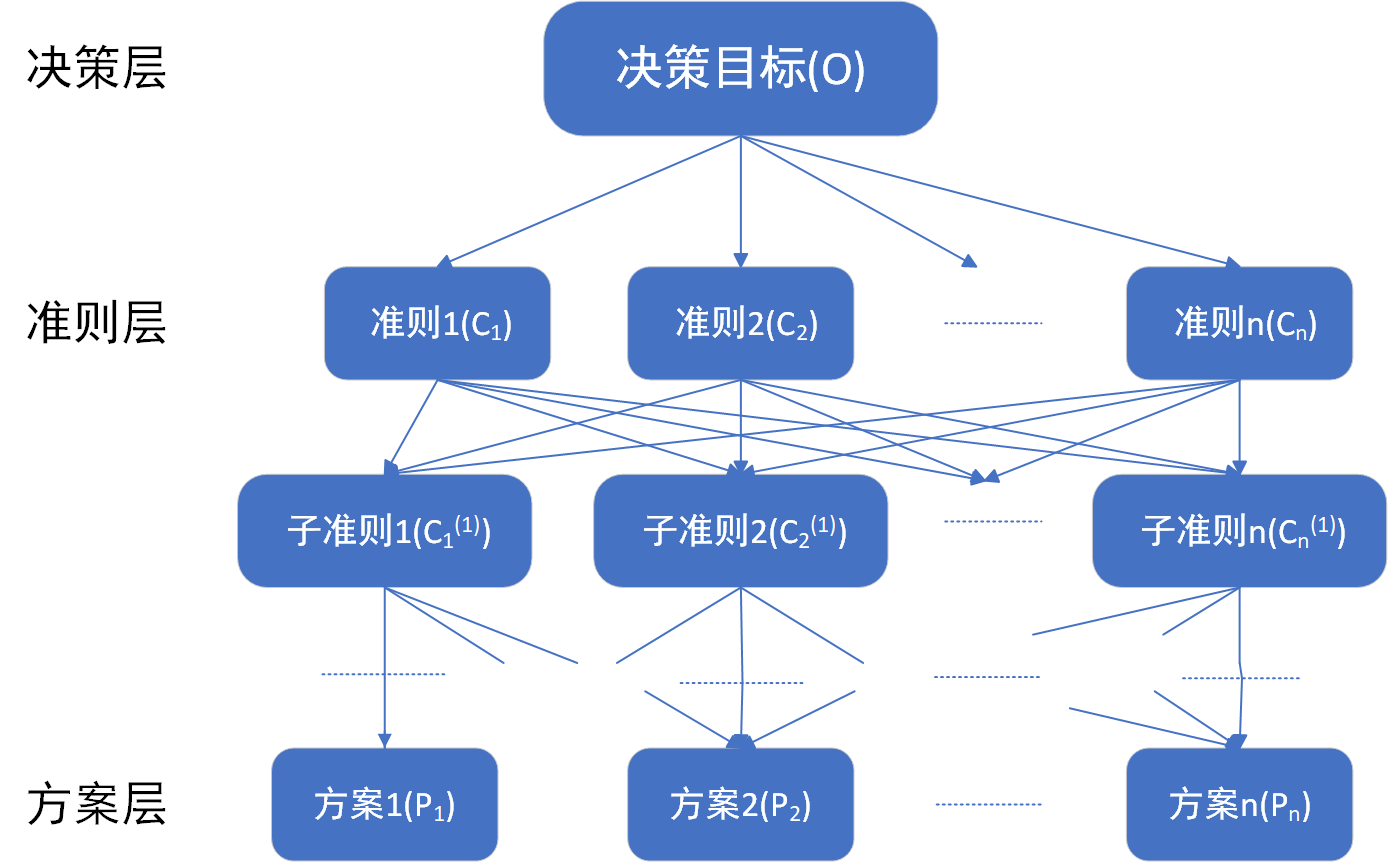
\includegraphics[height=4.5cm,width=9.5cm]{层次分析法框架.png}
                    \caption{层次分析法框架}
                \end{figure}
                准则层中准则因素之间相互独立。 \\
                我们选择的准则因素有:生活使用能耗、地区差异、周边产业、建造与拆除能耗、生产运输。

            \subsubsection{构建成对比较矩阵及归一化}
                \begin{enumerate}
                    \item 构建比较矩阵 \\
                        \qquad 构造比较矩阵是通过比较同一层次上的各因素对上–层相关因素的影响作用.而不是把所有因素放在一起比较,即将同一层的各因素进行两两对比。
                        设某层有n个因素,$ x = \{x_{1}, x_{2} \dots x_{n}\} $要比较它们对上一层某一准则 (或目标)的影响程度,确定在该层中相对于某一准则所占的比重。
                        上述比较是两两因素之间进行的比较,比较时常取1~9尺度。

                        \begin{table}[h]
                            \centering
                            \begin{tabular}{|c|c|} \hline
                                尺度 & 含义 \\ \hline
                                1 & 第i个因素与第j个因素影响相同 \\ \hline
                                3 & 第i个因素与第j个因素影响稍强 \\ \hline
                                5 & 第i个因素与第j个因素影响较强 \\ \hline
                                7 & 第i个因素与第j个因素影响明显强 \\ \hline
                                9 & 第i个因素与第j个因素影响极端强 \\ \hline
                                2, 4, 6, 8 & 两相邻判断的中间值 \\ \hline
                            \end{tabular}
                        \end{table}

                        用$ a_{ij} $表示第i个因素相对于第j个因素的比较结果,则
                        \[ a_{ij} = \frac{1}{a_{ji}} \]
                        \begin{equation}
                            A = (a_{ij})_{n \times n} =
                            \begin{pmatrix}
                                a_{11} & a_{12} & \cdots & a_{1n} \\
                                a_{21} & a_{22} & \cdots & a_{2n} \\
                                \cdots & \cdots & \cdots & \cdots \\
                                a_{n1} & a_{n2} & \cdots & a_{nn}
                            \end{pmatrix}
                        \end{equation}

                        A则称为成对比较矩阵。

                        \newpage


                        \item 归一化 \\
                            对各城市的数据进行归一化处理
                            \begin{table}[h]
                                \centering
                                \begin{tabular}[h]{|l|c|c|c|c|c|} \hline
                                    \diagbox{指标}{数据}{城市} & 苏州 & 南京 & 南通 & 无锡 & 常州 \\ \hline
                                    直接 & 48 & 51.5 & 27 & 57.2 & 29 \\ \hline
                                    间接 & 126.3 & 134.3 & 118.7 & 97.8 & 71.6 \\ \hline
                                    运营 & 4.8 & 4.9 & 3.5 & 2.7 & 2.8 \\ \hline
                                    \multirow{3}{*}{归一化比例} & 0.226 & 0.242 & 0.127 & 0.269 & 0.126 \\ \cline{2-6}
                                    ~ & 0.230 & 0.245 & 0.216 & 0.178 & 0.130 \\ \cline{2-6}
                                    ~ & 0.257 & 0.262 & 0.187 & 0.144 & 0.150 \\ \hline
                                \end{tabular}
                            \end{table}
                    \end{enumerate}


                \subsubsection{层次单排序及一致性检验}
                    \begin{enumerate}
                        \item 层次单排序 \\
                            和积法:取判断矩阵\textit{n}个列向量归一化后的算术平均值,近似作为权重,即
                            \begin{equation}
                                W_{i} = \frac{1}{n} \sum_{j=1}^{n} \frac{(\prod_{j=1}^{n} a_{ij})^{\frac{1}{n}}}{\sum_{k=1}^{n} (\prod_{j=1}^{n} a_{kj})^{\frac{1}{n}}} (i = 1, 2, \cdots, n)
                            \end{equation}

                            求根法(几何平均法):将比较矩阵的各列(或行)向量求几何平均后归一化,可近似作权重,即
                            \begin{equation}
                                W_{i} = \sum_{j=1}^{n} \frac{(\prod_{j=1}^{n} a_{ij})_{\frac{1}{n}}}{\sum_{k=1}^{n} (\prod_{j=1}^{n})_{\frac{1}{n}}} (i = 1, 2, \cdots, n)
                            \end{equation}

                            在我们的模型中综合采用了两种方法得到权重,降低了单一方法带来的不确定性,使数据结果更加可靠。


                        \item 一致性检验 \\
                        通常情况下,由实际得到的判断矩阵不一定是一致的,即不一定满足传递性和一致性实际中,也不必要求一致性绝对成立,
                        但要求大体上是一致的,即不一致的程度应在容许的范围内主要考查以下指标:
                            \begin{enumerate}
                                \item 一致性指标\textit{CI}
                                    \begin{equation}
                                        CI = \frac{\lambda _{\max} - n}{n - 1}
                                    \end{equation}

                                \item 平均随机一致性指标\textit{RI} \\
                                    为衡量\textit{CI}的大小,引入随机一致性指标\textit{RI}:
                                    \begin{equation}
                                        RI = \frac{CI_{1} + CI_{2} + \cdots + CI_{n}}{n}
                                    \end{equation}
                                    其中,随机一致性指标\textit{RI}和判断矩阵的阶数有关,一般情况下,
                                    矩阵阶数越大,则出现一致性随机偏离的可能性也越大,对于阶数小于9,其对应关系如图:
                                    \begin{table}[h]
                                        \centering
                                        \begin{tabular}{l|c c c c c c c c c} \hline
                                            \textit{n} & 1 & 2 & 3 & 4 & 5 & 6 & 7 & 8 & 9 \\ \hline
                                            \textit{RI} & 0 & 0 & 0.58 & 0.90 & 1.12 & 1.24 & 1.32 & 1.41 & 1.45 \\ \hline
                                        \end{tabular}
                                    \end{table}

                                \item 检验系数\textit{CR} \\
                                    考虑到一致性的偏离有可能是由于随机原因造成的,因此在检验判断矩阵是否具有满意的一致性时,
                                    还需将\textit{CI}和\textit{RI}进行比较,得出检验系数\textit{CR},公式如下:
                                    \begin{equation}
                                        CR = \frac{CI}{RI}
                                    \end{equation}
                                    一般地,如果$ CR \le 0.1 $,则认为该判断矩阵通过一致性检验,$ A_{\max} $对应的特征向量\textit{W}可以作为排序的权重向量,此时
                                    \begin{equation}
                                        \lambda _{\max} \approx \sum_{i=1}^{n} \frac{(A \cdot W)_{i}}{nw_{i}} = \frac{1}{n} \sum_{i=1}^{n} \frac{\sum_{j=1}^{n} a_{ij}w_{j}}{w_{i}}
                                    \end{equation}
                                    否则就不具有满意一致性,需要调整对比较矩阵。
                            \end{enumerate}
                    \end{enumerate}


                \subsubsection{计算组合权重及得分}
                    得到最大特征值对应的特征向量
                    \[ T = [t_1 \quad t_2 \quad \cdots \quad t_n] \]
                    \newline
                    计算得到权重向量
                    \[ W = [w_1 \quad w_2 \quad \cdots \quad w_n ] \]
                    \begin{equation*}
                        w_i = \frac{t_i}{\sum_{i=1}^{n} t_i}
                    \end{equation*}
                    \newline
                    设指标评分矩阵为\textit{P},那么最后的得分矩阵\textit{S}为:
                    \[ S = P \times W \]

    {\centering{\section{结果检验与误差分析}}}


    {\centering{\section{模型评价}}}


    {\centering{\section{模型推广与改进}}}


    {\centering{\section{参考文献}}}
    \newpage


    {\centering{\section{附录}}}
        \subsection*{附录A \hspace{2em} 问题一}
            \lstinputlisting[
                style       =   Python,
                caption     =   {\bf Question1},
                label       =   {Question1.py}
            ]{Question1.py}

        \subsection*{附录B \hspace{2em} 问题二}
            \lstinputlisting[
                style       =   Python,
                caption     =   {\bf Question2},
                label       =   {Question2.py}
            ]{Question2.py}

        \subsection*{附录C \hspace{2em} 问题三}

        \subsection*{附录D \hspace{2em} 问题四}

        \subsection*{附录E \hspace{2em} 问题五}

\end{document}
